\section{Complexity Theory}\label{sec:3}

\subsection{Polynomial Time Reduction}\label{subsec:3.1}
In practice, we can only solve problems that have polynomial time algorithms, 
since they can scale to large problems when the corresponding constants 
are small. We have polynomial time algorithms for shortest path, 
primality testing, and linear programming; in contrast, it is unlikely 
that there are polynomial time algorithms for longest path, factoring, 
and integer programming. We would like to classify problems into two 
categories: those that can be solved in polynomial time, and those that 
cannot be. But the bad news is that a huge number of fundamental 
problems have defied classification for decades. 

We introduce the notion of {\bf polynomial time reduction}.

\begin{defn}{defn:3.1}
    We say that problem $X$ {\bf reduces} to problem $Y$ in polynomial time if 
    arbitrary instances of problem $X$ can be solved using a polynomial number 
    of standard computational steps, plus a polynomial number of calls to 
    an oracle that solves problem $Y$. We write $X \leq_P Y$ in this scenario. 
\end{defn}

This definition allows us to do a few things. 
\begin{enumerate}[(1)]
    \item {\bf Design algorithms.} If $X \leq_P Y$ and $Y$ can be solved in 
    polynomial time, then $X$ can also be solved in polynomial time. 
    \item {\bf Establish intractability.} If $X \leq_P Y$ and $X$ cannot be 
    solved in polynomial time, then $Y$ cannot be solved in polynomial time. 
    \item {\bf Establish equivalence.} If $X \leq_P Y$ and $Y \leq_P X$, then 
    we write $X \equiv_P Y$. In this case, $X$ can be solved in polynomial 
    time if and only if $Y$ can be. 
\end{enumerate}
The bottom line is that reductions allow us to classify problems according 
to relative difficulty. 

We give two examples of polynomial time reductions here, and refer to Chapter 
8 of Kleinberg and Tardos for many other examples. 

Recall that a {\bf literal} is a boolean variable or its negation, and a 
{\bf clause} is a disjunction of literals. A propositional formula $\Phi$ is 
in {\bf conjunctive normal form (CNF)} if it is a conjunction of clauses. 
For example, $\Phi = (x_1 \vee \overline{x_2}) \wedge (\overline{x_1} 
\vee x_3)$ is in CNF. 

The {\sc Sat} problem is as follows: given a propositional formula $\Phi$ in 
CNF, does it have a satisfying truth assignment? Then the {\sc $3$-Sat} problem 
is {\sc Sat} where each clause contains exactly $3$ literals, and each literal 
corresponds to a different variable. This has a key application in electronic 
design automation. One example of an instance of {\sc $3$-Sat} is 
\[ \Phi = (\overline{x_1} \vee x_2 \vee x_3) \wedge (x_1 \vee \overline{x_2} 
\vee x_3) \wedge (\overline{x_1} \vee x_2 \vee x_4), \] 
which has a satisfying truth assignment of $x_1 = {\sf T}$, $x_2 = {\sf T}$, 
$x_3 = {\sf F}$, and $x_4 = {\sf F}$. 

The {\sc Independent-Set} problem is as follows: given a graph $G = (V, E)$ 
and an integer $k$, is there a subset of $k$ (or more) vertices such that 
no two are adjacent? It turns out that {\sc $3$-Sat} can be reduced to 
{\sc Independent-Set}. 

\begin{theo}{theo:3.2}
    We have $\textsc{3-Sat} \leq_P \textsc{Independent-Set}$.
\end{theo}
\begin{pf}
    Let $\Phi$ be an instance of {\sc $3$-Sat}. We will construct an instance 
    $(G, k)$ of {\sc Independent-Set} that has an independent set of size $k$ 
    if and only if $\Phi$ is satisfiable. 

    Let $G$ be a graph which contains $3$ nodes for each clause, one for 
    each literal. Connect the $3$ literals in a clause in a triangle, 
    and connect every literal to its negations. 

    For example, with $k = 3$ and $\Phi = (\overline{x_1} \vee x_2 \vee x_3) 
    \wedge (x_1 \vee \overline{x_2} \vee x_3) \wedge (\overline{x_1} \vee 
    x_2 \vee x_4)$ as above, we can see that $G$ will be the following graph. 

    \begin{center}
        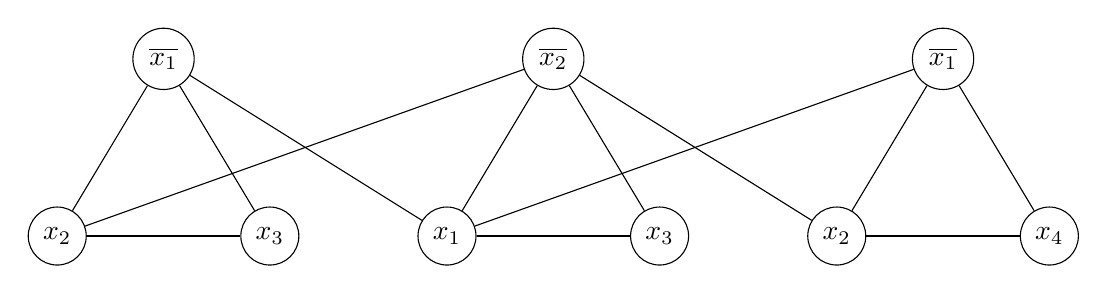
\begin{tikzpicture}  
          [scale=.9,auto=center,every node/.style={circle,draw=black}] % here, node/.style is the style pre-defined, that will be the default layout of all the nodes. You can also create different forms for different nodes.  
              
            \node (1) at (5, 2.5) {$\overline{x_1}$};  
            \node (2) at (3.5, 0) {$x_2$};  
            \node (3) at (6.5, 0) {$x_3$};

            \node (4) at (10.5, 2.5) {$\overline{x_2}$};
            \node (5) at (9, 0) {$x_1$};
            \node (6) at (12, 0) {$x_3$};

            \node (7) at (16, 2.5) {$\overline{x_1}$};
            \node (8) at (14.5, 0) {$x_2$};
            \node (9) at (17.5, 0) {$x_4$};
    
            \draw (1) -- (2);
            \draw (1) -- (3);
            \draw (2) -- (3);

            \draw (4) -- (5);
            \draw (4) -- (6);
            \draw (5) -- (6);

            \draw (7) -- (8);
            \draw (7) -- (9);
            \draw (8) -- (9);

            \draw (1) -- (5);
            \draw (5) -- (7);
            \draw (2) -- (4);
            \draw (4) -- (8);
            
        \end{tikzpicture} 
    \end{center}
    We claim that $\Phi$ is satisfiable if and only if $G$ contains 
    an independent set of size $k = |\Phi|$. 

    For the forward direction, consider any satisfying assignment for $\Phi$. 
    Then selecting one true literal from each clause (or triangle) will 
    give an independent set of size $k$. 

    Conversely, let $S$ be an independent set of size $k$. Then $S$ must 
    contain exactly one node in each triangle by construction. Set these 
    literals to ${\sf T}$ (and the remaining literals consistently). Then 
    all clauses in $\Phi$ are satisfied. This completes the proof. 
\end{pf}

The {\sc Vertex-Cover} problem is the following: given a graph $G = (V, E)$ 
and an integer $k$, is there a subset of $\leq k$ vertices such that 
each edge is incident to at least one vertex in the subset? 

The {\sc Set-Cover} problem is the following: given a set $U$ of elements, 
a collection $S$ of subsets of $U$, and an integer $k$, are there $\leq k$ 
of these subsets whose union is equal to $U$? 

\begin{theo}{theo:3.3}
    We have $\textsc{Vertex-Cover} \leq_P \textsc{Set-Cover}$. 
\end{theo}
\begin{pf}
    Given a {\sc Vertex-Cover} instance with the graph $G = (V, E)$ and 
    integer $k$, we construct a {\sc Set-Cover} instance $(U, S, k)$ that 
    has a set cover of size $k$ if and only if $G$ has a vertex cover of 
    size $k$. 

    We do this by setting the universe to be $U = E$, and include a 
    subset for each node $v \in V$ by 
    \[ S_v = \{e \in E : e \text{ incident to } v\}. \] 
    For example, consider the following graph $G$, which has a vertex 
    cover of size $2$ given by $\{c, f\}$. 
    \begin{center}
        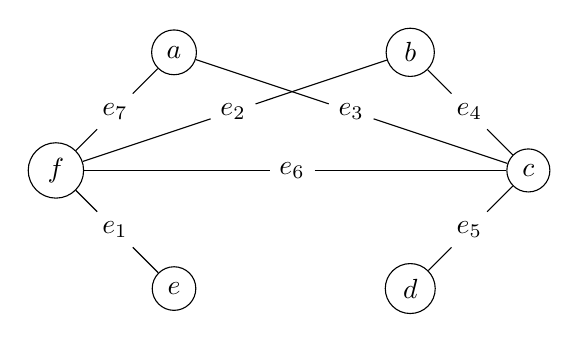
\begin{tikzpicture}              
            \node [circle, draw=black] (a) at (5, 3) {$a$};  
            \node [circle, draw=black] (b) at (8, 3) {$b$}; 
            \node [circle, draw=black] (c) at (9.5, 1.5) {$c$}; 
            \node [circle, draw=black] (d) at (8, 0) {$d$}; 
            \node [circle, draw=black] (e) at (5, 0) {$e$}; 
            \node [circle, draw=black] (f) at (3.5, 1.5) {$f$};

            \node (e1) at (4.25, 0.75) {$e_1$};
            \node (e2) at (5.75, 2.25) {$e_2$};
            \node (e3) at (7.25, 2.25) {$e_3$};
            \node (e4) at (8.75, 2.25) {$e_4$};
            \node (e5) at (8.75, 0.75) {$e_5$};
            \node (e6) at (6.5, 1.5) {$e_6$};
            \node (e7) at (4.25, 2.25) {$e_7$};

            \draw (e) -- (e1) -- (f);
            \draw (f) -- (e2) -- (b);
            \draw (a) -- (e3) -- (c);
            \draw (b) -- (e4) -- (c);
            \draw (c) -- (e5) -- (d);
            \draw (f) -- (e6) -- (c);
            \draw (f) -- (e7) -- (a);           
        \end{tikzpicture} 
    \end{center}
    Then we have universe $U = \{1, 2, 3, 4, 5, 6, 7\}$ with subsets 
    $S_a = \{3, 7\}$, $S_b = \{2, 4\}$, $S_c = \{3, 4, 5, 6\}$, 
    $S_d = \{5\}$, $S_e = \{1\}$, and $S_f = \{1, 2, 6, 7\}$. We can 
    see that $U = S_c \cup S_f$, so there is a set cover of size $2$. 

    Let us now show that $G = (V, E)$ contains a vertex cover of size $k$ 
    if and only if $U$ has a set cover of size $k$. 

    For the forward direction, let $X \subseteq V$ be a vertex cover of 
    size $k$ in $G$. Then $Y = \{S_v : v \in X\}$ is a set cover of size $k$. 
    Conversely, if $Y \subseteq S$ is a set cover of size $k$ for $U$, then 
    $X = \{v : S_v \in Y\}$ is a vertex cover of size $k$ in $G$. 
\end{pf}

\subsection{Intractability}\label{subsec:3.2}
There are three main types of problems. 
\begin{itemize}
    \item {\bf Decision problems.} Does there \emph{exist} a vertex cover of 
    size $\leq k$?
    \item {\bf Search problems.} \emph{Find} a vertex cover of size $\leq k$. 
    \item {\bf Optimization problems.} \emph{Find} a vertex cover of 
    \emph{minimum} size. 
\end{itemize}
In scheduling, we are mostly concerned with optimization problems. Notice that 
decision problems are in some sense easier than search problems, which are then 
easier than optimization problems. In particular, if the decision problem 
is intractible, then both the search and optimization problems are intractible.
Because of this, we will define {\bf P}, {\bf NP}, and {\bf EXP} using decision 
problems. A decision problem is essentially a yes or no question; we want to 
answer ``yes'' if the solution exists and ``no'' if it doesn't. 

\begin{defn}{defn:3.4}
    We denote by ${\bf P}$ the set of decision problems for which there 
    exists a polynomial time algorithm to solve it. 
\end{defn}

As we mentioned earlier, there are polynomial time algorithms for shortest 
path, primality testing, and linear programming, so these problems are all 
in {\bf P}. 

\begin{defn}{defn:3.5}
    \begin{itemize}
        \item An algorithm $C(s, t)$ is a {\bf certifier} for the problem $X$ if 
        for every string $s$, we have $s \in X$ if and only if there exists a 
        string $t$ such that $C(s, t)$ returns ``yes''. We call the string $t$ 
        the {\bf certificate} for the input $s$. 
        \item We denote by {\bf NP} the set of decision problems for which there exists 
        a polynomial time certifier. The certifier $C(s, t)$ is a 
        polynomial time algorithm, and the certificate $t$ for the input 
        $s$ is of polynomial size. 
    \end{itemize}
\end{defn}

\begin{exmp}{exmp:3.6}
    For the {\sc Sat} and {\sc 3-Sat} problems, the input is a propositional 
    formula $\Phi$ in CNF. A certificate for the input $\Phi$ is an 
    assignment of truth values to the boolean variables, and a certifier 
    checks that each clause in $\Phi$ has at least one true literal. 
    Thus, $\textsc{Sat} \in {\bf NP}$ and $\textsc{3-Sat} \in {\bf NP}$. 
\end{exmp}

Finally, we can define {\bf EXP}. 

\begin{defn}{defn:3.7}
    We denote by {\bf EXP} the set of decision problems for which there 
    exists an exponential time algorithm to solve it.
\end{defn}

\newpage
Now, we show that $\Poly \subseteq \NP \subseteq \EXP$. 

\begin{prop}{prop:3.8}
    We have $\Poly \subseteq \NP$. 
\end{prop}
\begin{pf}
    Consider a problem $X$ in $\Poly$. By definition, there exists a 
    polynomial time algorithm $A(s)$ which solves $X$ given any input $s$. 
    Then take the certificate $t = \eps$ to be the empty string, and 
    set the certifier to be $C(s, t) = A(s)$, which of course runs 
    in polynomial time. 
\end{pf}

\begin{prop}{prop:3.9}
    We have $\NP \subseteq \EXP$. 
\end{prop}
\begin{pf}
    Let $X$ be a problem in $\NP$. By definition, there exists a polynomial 
    time certifier $C(s, t)$ for $X$, whose certificate $t$ satisfies 
    $|t| \leq p(|s|)$ for some polynomial $p$ and any input string $s$. 
    To solve instance $s$, we run $C(s, t)$ on all strings $t$ with 
    $|t| \leq p(|s|)$. Return ``yes'' if and only if $C(s, t)$ returns 
    ``yes'' for any of these potential certificates. 
\end{pf}

It is a known fact that $\Poly \neq \EXP$, so we either have $\Poly \neq \NP$ 
or $\NP \neq \EXP$, or both. 

We now move on to {\bf NP}-completeness. We can think of these as the 
hardest problems in $\NP$. 

\begin{defn}{defn:3.10}
    A problem $Y \in \NP$ is called {\bf $\NP$-complete} if it has the property 
    that for every $X \in \NP$, we have $X \leq_P Y$. 
\end{defn}

The following proposition says that if we find even one problem $\NP$-complete 
problem $Y$ that is also in $\Poly$, then $\Poly = \NP$. Note that $\Poly = \NP$ 
is a famous conjecture, so we have of course not found one yet. It is commonly 
agreed upon that $\Poly \neq \NP$, but it is still an open problem.

\begin{prop}{prop:3.11}
    Suppose that $Y$ is $\NP$-complete. Then $Y \in \Poly$ if and only if 
    $\Poly = \NP$. 
\end{prop}
\begin{pf}
    For the backwards direction, notice that if $\Poly = \NP$, then 
    $Y \in \Poly$ since $Y \in \NP$. On the other hand, suppose $Y \in \Poly$. 
    Consider any problem $X \in \NP$. Since $X \leq_P Y$, we have $X \in \Poly$. 
    This implies that $\NP \subseteq \Poly$, and so $\Poly = \NP$. 
\end{pf}

The following proposition gives us a recipe for proving that a problem $Y$ 
is $\NP$-complete. 
\begin{enumerate}
    \item Show that $Y \in \NP$. 
    \item Choose an $\NP$-complete problem $X$ and prove that $X \leq_P Y$. 
\end{enumerate}

\begin{prop}{prop:3.12}
    If $X$ is $\NP$-complete, $Y \in \NP$, and $X \leq_P Y$, then 
    $Y$ is also $\NP$-complete. 
\end{prop}
\begin{pf}
    Consider any problem $W \in \NP$. Then $W \leq_P X$ by the definition 
    of $\NP$-completeness and $X \leq_P Y$ by assumption, so by transitivity, 
    we obtain $W \leq_P Y$. Since $W \in \NP$ is arbitrary, we have 
    that $Y$ is $\NP$-complete. 
\end{pf}

We now give some examples of $\NP$-complete problems. It is useful to know 
them as many scheduling problems are $\NP$-complete, and we can verify 
that they are indeed $\NP$-complete via reductions. 

\begin{theo}[Cook 1971, Levin 1973]{theo:3.13}
    The problem {\sc Sat} is $\NP$-complete. 
\end{theo}

\begin{exmp}{exmp:3.14}
    The following two problems are $\NP$-complete. 
    \begin{itemize}
        \item {\sc Partition}: Given $n$ positive integers $s_1, \dots, s_n$ 
        and $b = \frac12 \sum_{j=1}^n s_j$, does there exist a subset 
        $J \subseteq I = \{1, \dots, n\}$ such that 
        \[ b = \sum_{j\in J} s_j = \sum_{j\in I\setminus J} s_j? \] 
        \item {\sc $3$-Partition}: Given $3n$ positive integers 
        $s_1, \dots, s_{3n}$, and an integer $b$ satisfying 
        $\frac{b}{4} < s_j < \frac{b}{2}$ for all $j \in \{1, \dots, 3n\}$ 
        and $b = \frac1n \sum_{j=1}^{3n} s_j$, do there exist 
        $n$ pairwise disjoint three-element subsets $S_j \subseteq 
        \{1, \dots, 3n\}$ such that 
        \[ b = \sum_{j\in J_i} s_j \] 
        for all $j \in \{1, \dots, n\}$? 
    \end{itemize}
\end{exmp}

Next, we define what it means to be $\NP$-hard. 

\begin{defn}{defn:3.15}
    An $\NP$-hard problem is one such that every problem in $\NP$ 
    reduces to it in polynomial time. 
\end{defn}

Intuitively, $\NP$-hard problems are ``at least as hard as the hardest 
problems in $\NP$''. These problems are not necessarily in $\NP$, and they 
do not have to be decision problems. 
For instance, given an $\NP$-complete decision problem, the optimization 
problem corresponding to it is $\NP$-hard. 

There are two categories of $\NP$-hard problems.  
\begin{itemize}
    \item {\bf NP-hard in the ordinary sense.} We can reduce a known 
    $\NP$-hard problem to this problem using a polynomial time algorithm, 
    and we can find an optimal solution with an algorithm of pseudo-polynomial 
    time complexity. 
    \item {\bf NP-hard in the strong sense.} We can reduce a known 
    $\NP$-hard problem to this problem using a polynomial time algorithm, 
    even if the size of the largest parameter is polynomial in the 
    input size of the problem. 
\end{itemize}

In fact, it turns out that {\sc 3-Partition} (as defined in Example~\ref{exmp:3.14})
is $\NP$-hard in the strong sense, while {\sc Partition} is only $\NP$-hard 
in the ordinary sense. 

For our purposes, we can show that a scheduling problem is $\NP$-hard 
in the ordinary sense if {\sc Partition} (or a similar problem) can be 
reduced to this problem with a polynomial time algorithm, and there 
is an algorithm with pseudo-polynomial time complexity which solves the 
scheduling problem. 

On the other hand, we can show that a scheduling problem is $\NP$-hard 
in the strong sense if {\sc 3-Partition} (or a similar problem) can be 
reduced to this problem with a polynomial time algorithm. 

\subsection{PTAS for the Knapsack Problem}\label{subsec:3.3}
A {\bf polynomial time approximation scheme (PTAS)} is a
$(1 + \eps)$-approximation algorithm for any constant $\eps > 0$. 
While a PTAS produces arbitrarily high quality solutions, the consequence 
is that it trades off accuracy for time. Here, we will give a PTAS for the 
{\sc Knapsack} problem via rounding and scaling. 

In the {\sc Knapsack} problem, we are given $n$ objects and a knapsack. 
Each item $i$ has value $v_i > 0$ and weight $w_i > 0$. The knapsack 
has weight limit $W$. The goal is to fill the knapsack as to maximize 
the total value. 

First, we formulate the {\sc Knapsack} problem as a decision problem
and give a brief sketch that it is $\NP$-complete. 
Given a set $X$, weights $w_i \geq 0$, values $v_i \geq 0$, a weight 
limit $W$, and a target value $V$, is there a subset $S \subseteq X$ 
such that $\sum_{i\in S} w_i \leq W$ and $\sum_{i\in S} v_i \geq V$? 

The {\sc Subset-Sum} problem is the following: given $n$ natural numbers 
$w_1, \dots, w_n$ and an integer $W$, is there a subset that adds up to 
exactly $W$?

We know that {\sc Sat} is $\NP$-complete, and one can show that 
\[ \textsc{Sat} \leq_P \textsc{Subset-Sum} \leq_P \textsc{Knapsack}. \] 
